\section{Policy Refactoring} \label{sec:approach}
This section describes our approach of refactoring access control policies to improve performance by reducing the number of policy 
rules potentially applicable to a request. For refactoring policies in a systematic way, we propose seven policy splitting 
criteria based on attribute sets. 
Moreover, we explain how to select a splitting criterion that preserves the synergy in the access control architecture.

\subsection{Policy Splitting Criteria} \label{subsec:SplittingCriteria}
Given a request, a PDP typically uses brute force searching to determine a decision by evaluating the request against all the policy rules 
one by one until the PDP finds a decision.

During the evaluation process, the attribute values in a given request are compared with the attribute in the target of a rule. 
If there is a match between the request's attribute and target's attribute values, the rule is then applicable to the request.
In decision making process, applicable rules contribute
to build the final authorization decision whereas non-applicable rules are not relevant in this process. 
For request evaluation, not all the rules are applicable to the request. In other words, only part of the rules (i.e, relevant rules) are
 applicable to the request and can contribute to determining the final decision.

We propose an approach to evaluate a request against only the relevant rules for the given request by refactoring the access control policies. Our approach aims at splitting a single global policy into 
multiple smaller policies based on attribute combination. For a given policy-based system, we transform its policy \normalsize $P$ into 
policies \normalsize $P_{SC_{w}}$ containing a less number of rules and conforming to a Splitting Criterion $SC_{w}$. 
An $SC_{w}$ defines the set of attributes that are considered to classify all the rules into subsets each with the same attribute values and $w$ denotes 
the number of attributes that have to be considered conjointly for aggregating rules based on specific attribute elements. 
Table \ref{table1} 
shows our proposed splitting criteria categorized according to attribute element combinations.
\begin{table}[h!]
\centering
\setlength{\extrarowheight}{6 pt}
\begin{tabular}{|>{\small}c|>{\small}c|}
\hline \rowcolor{black}
\bf
\textcolor{white}{Categories}& \bf \textcolor{white}{Splitting Criteria}\\ \hline
$SC_{1}$& {$\langle Subject \rangle, \langle Resource\rangle, \langle Action\rangle$}\\ \hline
$SC_{2}$& {$\langle Subject,Action \rangle, \langle Subject,Resource\rangle$}\\&{$\langle Resource,Action\rangle$}\\ \hline
$SC_{3}$& {$\langle Subject,Resource,Action\rangle$}\\ \hline
\end{tabular}
\caption{Splitting Criteria}
\label{table1}\end{table}

To illustrate our approach, we present examples that take into consideration the XACML language features.
In Figure \ref{splitting}, our approach refactors an XACML policy $P$  according to the splitting criterion $SC_{1}=\langle Subject\rangle$. Our refactoring results 
in two sub-policies $Pa$ and $Pb$. Each sub-policy consists of relevant rules with regards to the same subject (Alice or Bob in this case). 

\begin{figure}[!h]
\begin{center}
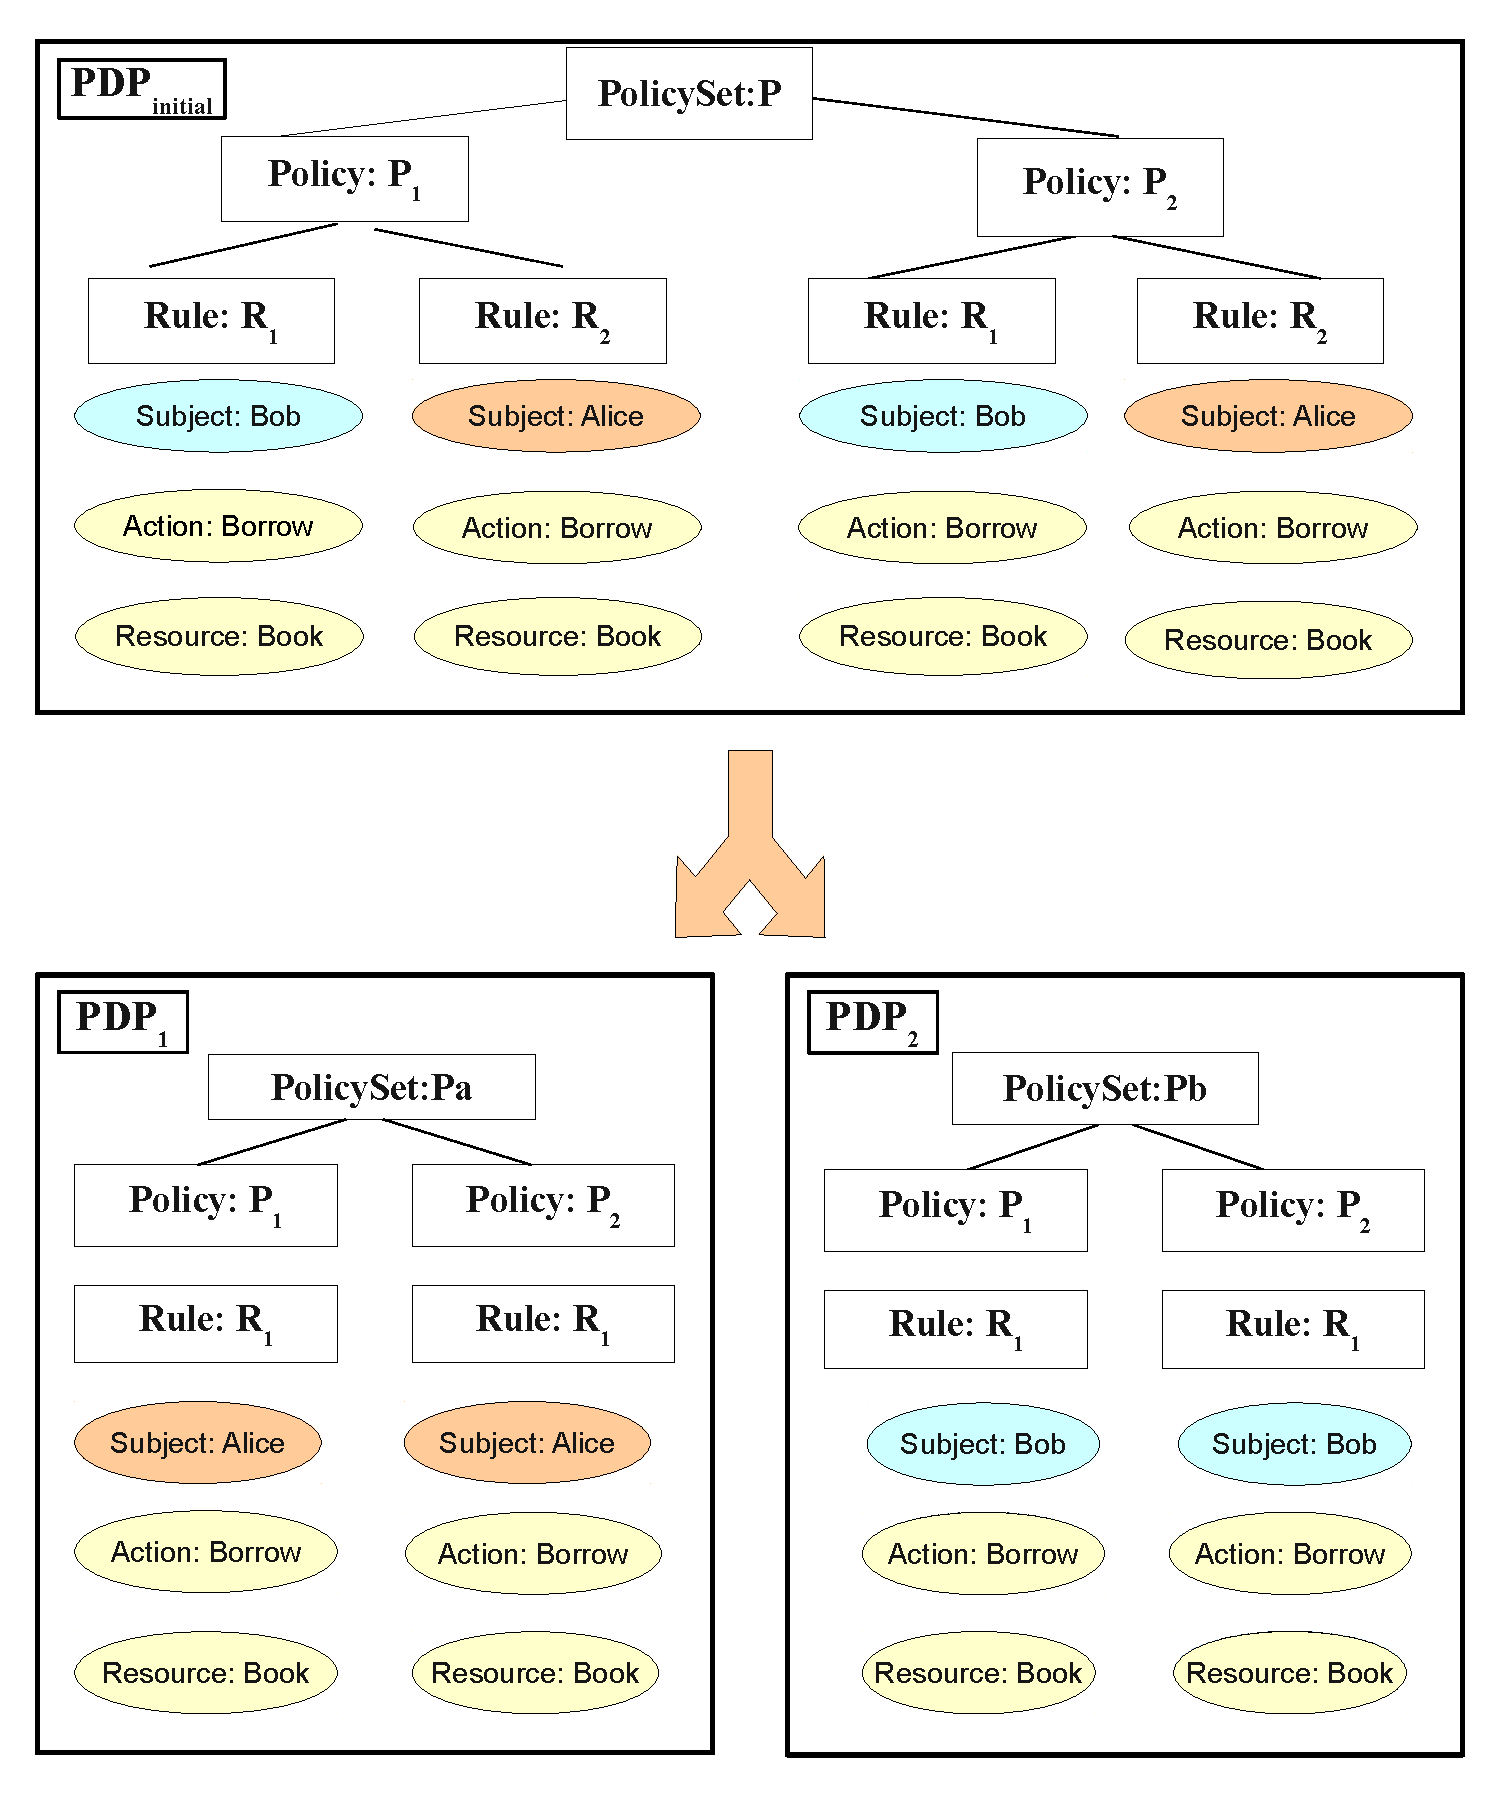
\includegraphics[width=8.5cm, height=10cm]{splitting}
\caption{Refactoring a policy according to $SC_{1}=\langle Subject\rangle$}
\label{splitting}
\end{center}
\end{figure}

Technically, to split a given policy $P$ according to $SC_{1}=\langle Subject\rangle$, we start by parsing the global policy $P$ 
and by collecting the overall subject attributes in the policy. For each collected subject attribute $Sa$, we consider the global policy and we 
delete the rules that do not contain $Sa$ as a subject attribute in the target element attributes. After all the successive deletions, the global 
policy is refactored to a policy that contains only the rules with $Sa$ in their subject attribute elements. 
Algorithm 1 shows the algorithm about the splitting process for $SC_{1}=\langle Subject\rangle$.

\begin{algorithmic}
\begin{algorithm}[t]
\caption{Policy Splitting Algorithm}
\STATE \textbf{Input:} XACML Policy $P$, Splitting Criterion $SC_{1}$=$\langle Subject \rangle$
\STATE \textbf{Output:} Sub-policies Set: S
\STATE \textbf{SplitPolicy()}
\STATE {S=\O{}}
\STATE /* Collect all subjects in all the rules /*
\FORALL{Rule $R_{i}$ in Policy $P$}
\STATE /* Fetch all the targets to extract attribute collection depending on $SC$ */
\FORALL{Target.Subject in $R_{i}$}
\STATE SubjectCollection.add(SubjectElement.attribute)
\ENDFOR
\ENDFOR
\STATE /* Build sub-policies based on subjects collected in SubjectCollection */
\FOR{int $i = 0$; $i$ $<$ SubjectCollection.size(); $i++$}
\STATE /* Remove all the rules that do not contain SubjectCollection.at(i) in their Target */
\FORALL{Rule $R_{i}$ in Policy $P$}
\IF {$R_{i}.Target.SubjectElement$ \textbf{$!=$} AnySubject}
\IF {(Target.SubjectElement.attribute in $R_{i}$) \textbf{$!=$} SubjectCollection.at(i)}
\STATE{Remove $R_{i}$}\ENDIF 
\ENDIF
\ENDFOR
\STATE /* $P_{(SubjectCollection.at(i))}$ is a sub-policy with only rules where the subjectAttribute is equal to SubjectCollection.at(i) */
\STATE /* Add the sub-policy to the set of sub-policies */
\STATE $S=S \cup P_{(SubjectCollection.at(i))}$
\ENDFOR
\end{algorithm}
\end{algorithmic}

%%%%%%%%%%%%%%%%%%%%%%%%%%%%%%%%%%%%%%%%%%%%%%%%Discussion on safety%%%%%%%%%%%%%%%%%%%%%%%%%%%%
Our algorithm is safe in the sense that it does not change the authorization behavior of the PDP. 
There are two important issues to be considered when reasoning about the safety of the algorithm:
\begin{itemize}
 \item Can the splitting impact authorization results when a policy set includes multiple policies with different combining algorithms?
 \item When 'AnySubject', 'AnyAction', 'AnyResource' is used as target element values, does the splitting change the behavior of the PDP?
\end{itemize}
The first issue is addressed by the way the algorithm operates. The first step of the algorithm goes through all the rules and extracts 
depending on the splitting criterion, the set of target elements (the set of subjects, 
the set of actions, and/or the set of resources). Then, based on the extracted result, the splitting is performed by removing 
the rules with different splitting criterion values (such as a subject different from 
the splitting criterion subject). The rules that are kept are therefore not modified and therefore their behavior is not altered. When there 
are several policies with different combining algorithms, the rules that are kept do not impact the evaluation behavior 
because they remain attached to the same combining algorithm. Moreover their order and their content are not modified.


The second issue is handled by keeping all the rules that involve 'AnySubject', 'AnyAction' or 'AnyResource' because by definition during 
evaluation, these values are taken into consideration for evaluating all possible values of subjects, actions, and resources. 
Therefore, it is important to keep them in all split policies because they are used in all evaluations, this way, the behavior is not changed because these rules are present in all split policies and 
their number is negligible compared to those existing in specific targets. 


%%%%%%%%%%%%%%%%%%%%%%%%%%%%%%%%%%%%%%%%%%%%%%%%%%%%%%%%%%%%%%%%%%%%%%%%%%
It is worth mentioning this following consideration related to the refactoring process:
XACML supports multi-valued attributes in policies and requests. In XACML policies, \CodeIn{target} elements define a set of attribute values, which match with 
the context element in 
an access control request. In Figure \ref{xacml-match}, the subject attribute includes two attributes (one is ``role'' and the other 
is ``isEq-subjUserId-resUserId``). In order to match the subject with multi-valued attributes, a request should include at least \CodeIn{pc-member} and \CodeIn{ture} 
for ''role`` and ''isEq-subjUserId-resUserId``, respectively.
Our approach considers such a whole subject element as a single entity, which is not split by the policy splitter component.
\begin{figure}[!h]
\begin{center}
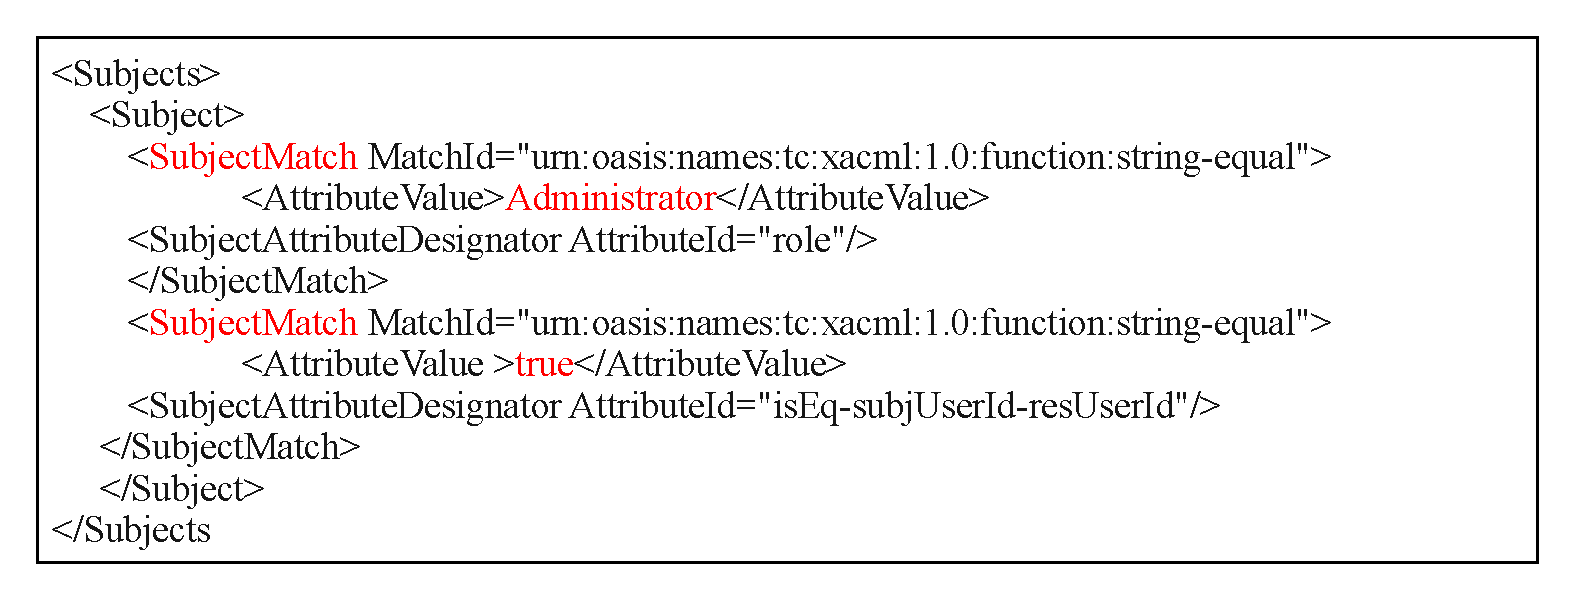
\includegraphics[width=9cm, height=3.5cm]{xacml-match}
\caption{Multi-attribute values in \CodeIn{target} element}
\label{xacml-match}
\end{center}
\end{figure}

After the splitting is performed, our approach creates one or more PDPs that comply with the splitting criterion.
We use Sun PDP \cite{sunxacml} to evaluate requests against policies specified in XACML.
During request evaluation, Sun PDP checks the request against the policy and determines whether the
decision is permit or deny. Given a request, our approach runs Sun PDP loaded with the request's relevant policy,
 which is used during the decision making process. The PDP then retrieves the rules that are applicable to the request.
Figure \ref{requestevaluation} presents our approach to handling request evaluation with multiple policies. 
During the evaluation process, given a request, our approach verifies the matching between the request's attribute values, 
and the policy target elements attributes. Our approach then selects only the relevant policy among all the policies for a given request.
After the selection of the relevant policy, all of its relevant rules for the decision making are evaluated.

\begin{figure}[!h]
\begin{center}
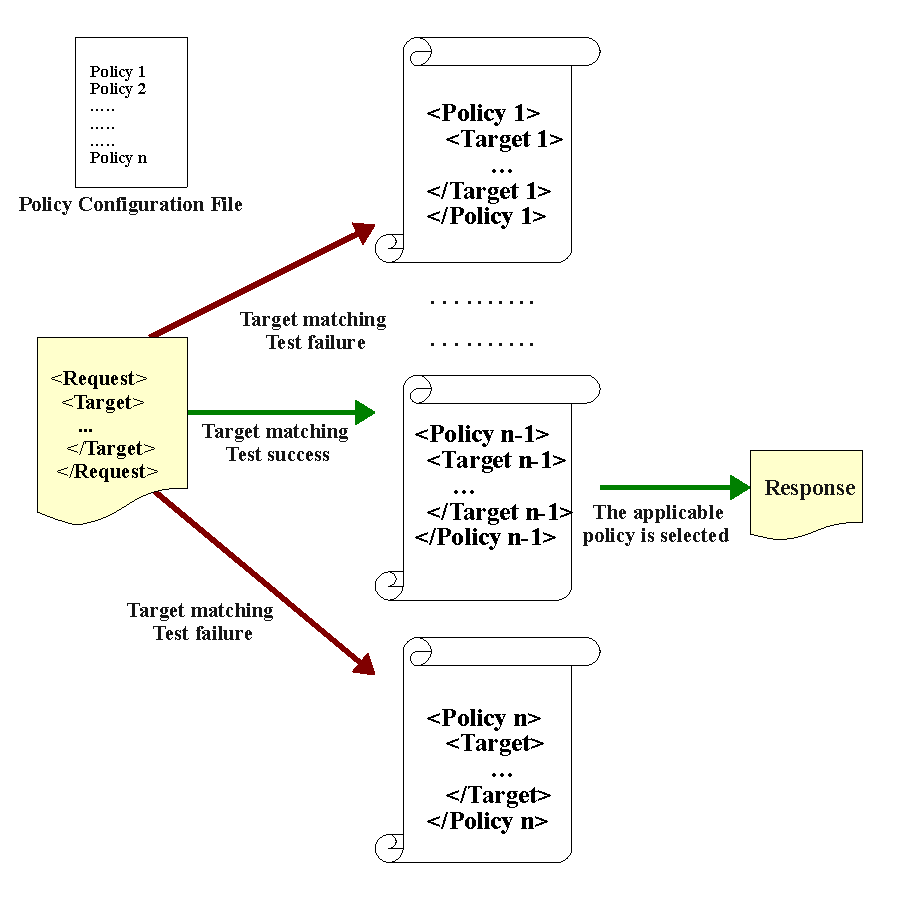
\includegraphics[width=3in, height=3in]{requestevaluation}
\caption{Applicable-Policy Selection}
\label{requestevaluation}
\end{center}
\end{figure}


Figure \ref{overallprocess} shows an overview of our approach.
In our approach, the policy splitter component plays a role to refactor access control policies.
Given a single PDP loaded with the initial global policy, the policy splitter component conducts automated refactoring 
by creating multiple PDPs loaded with XACML policies, which are split from the initial global policy based on the user-specified splitting criterion. 
%Afterwards, the policies are included in the 
%framework that supports our approach. 
If the initial global policy is changed, the policy splitter component is required to refactor the policy again to create PDPs with the most recent relevant policies.
Our refactoring approach is safe in the sense that the approach does not impact existing security aspects in a given
system. 


\begin{figure}[!h]
\begin{center}
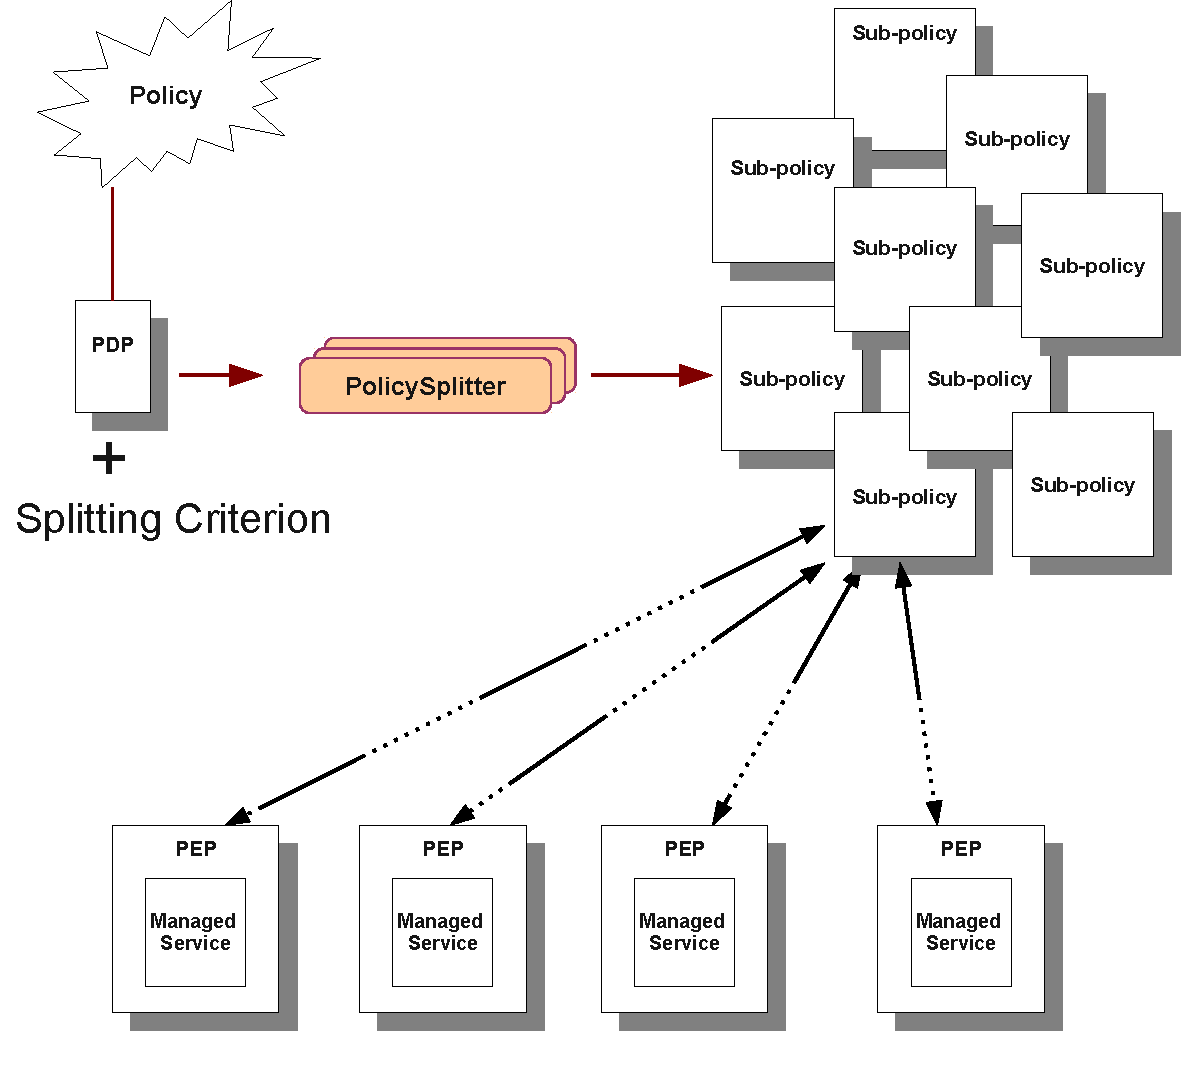
\includegraphics[width=8.5cm, height=8cm]{Overall-process}
\caption{Overview of the Refactoring Process}
\label{overallprocess}
\end{center}
\end{figure}


\subsection{Architecture Model Preservation: PEP-PDP Synergy}

We propose to preserve the synergy requirement in the access control architecture by mapping a PEP and a PDP loaded
with the relevant policy for a request dynamically at runtime. As shown in Section \ref{subsec:SplittingCriteria}, given multiple PDPs after the policy refactoring, we consider 
(1) how PEPs are organized at the application level, and (2) how PEPs are linked to their corresponding PDPs.
In the worst case, splitting the initial PDP into multiple PDPs may lead to a non-synergic system: a PEP may send its requests to several PDPs. 
The PDP, that handles a given request is only known at runtime. Such a resulting architecture breaks the PEP-PDP synergy and the conceptual 
simplicity of the initial architecture model. 
In the best case, the refactoring preserves the simplicity of the initial architecture by keeping a many-to-one association 
between PEPs to PDPs. Given a request, our approach maps a PEP to a PDP with relevant rules for the request.
Threfore, different requests issued from a PEP should be handled by the same PDP. Operationally, the request evaluation involves 
one policy. In this case, our refactoring does not impact the conceptual architecture of the system.

Figure \ref{Synergicvsnonsynergicarchitecture} presents a PDP encapsulating a global policy that has been refactored. The system that is 
presented on the left is a desirable refactoring whereas the one on the right shows an undesirable refactoring.
\begin{figure}[!h]
\begin{center}
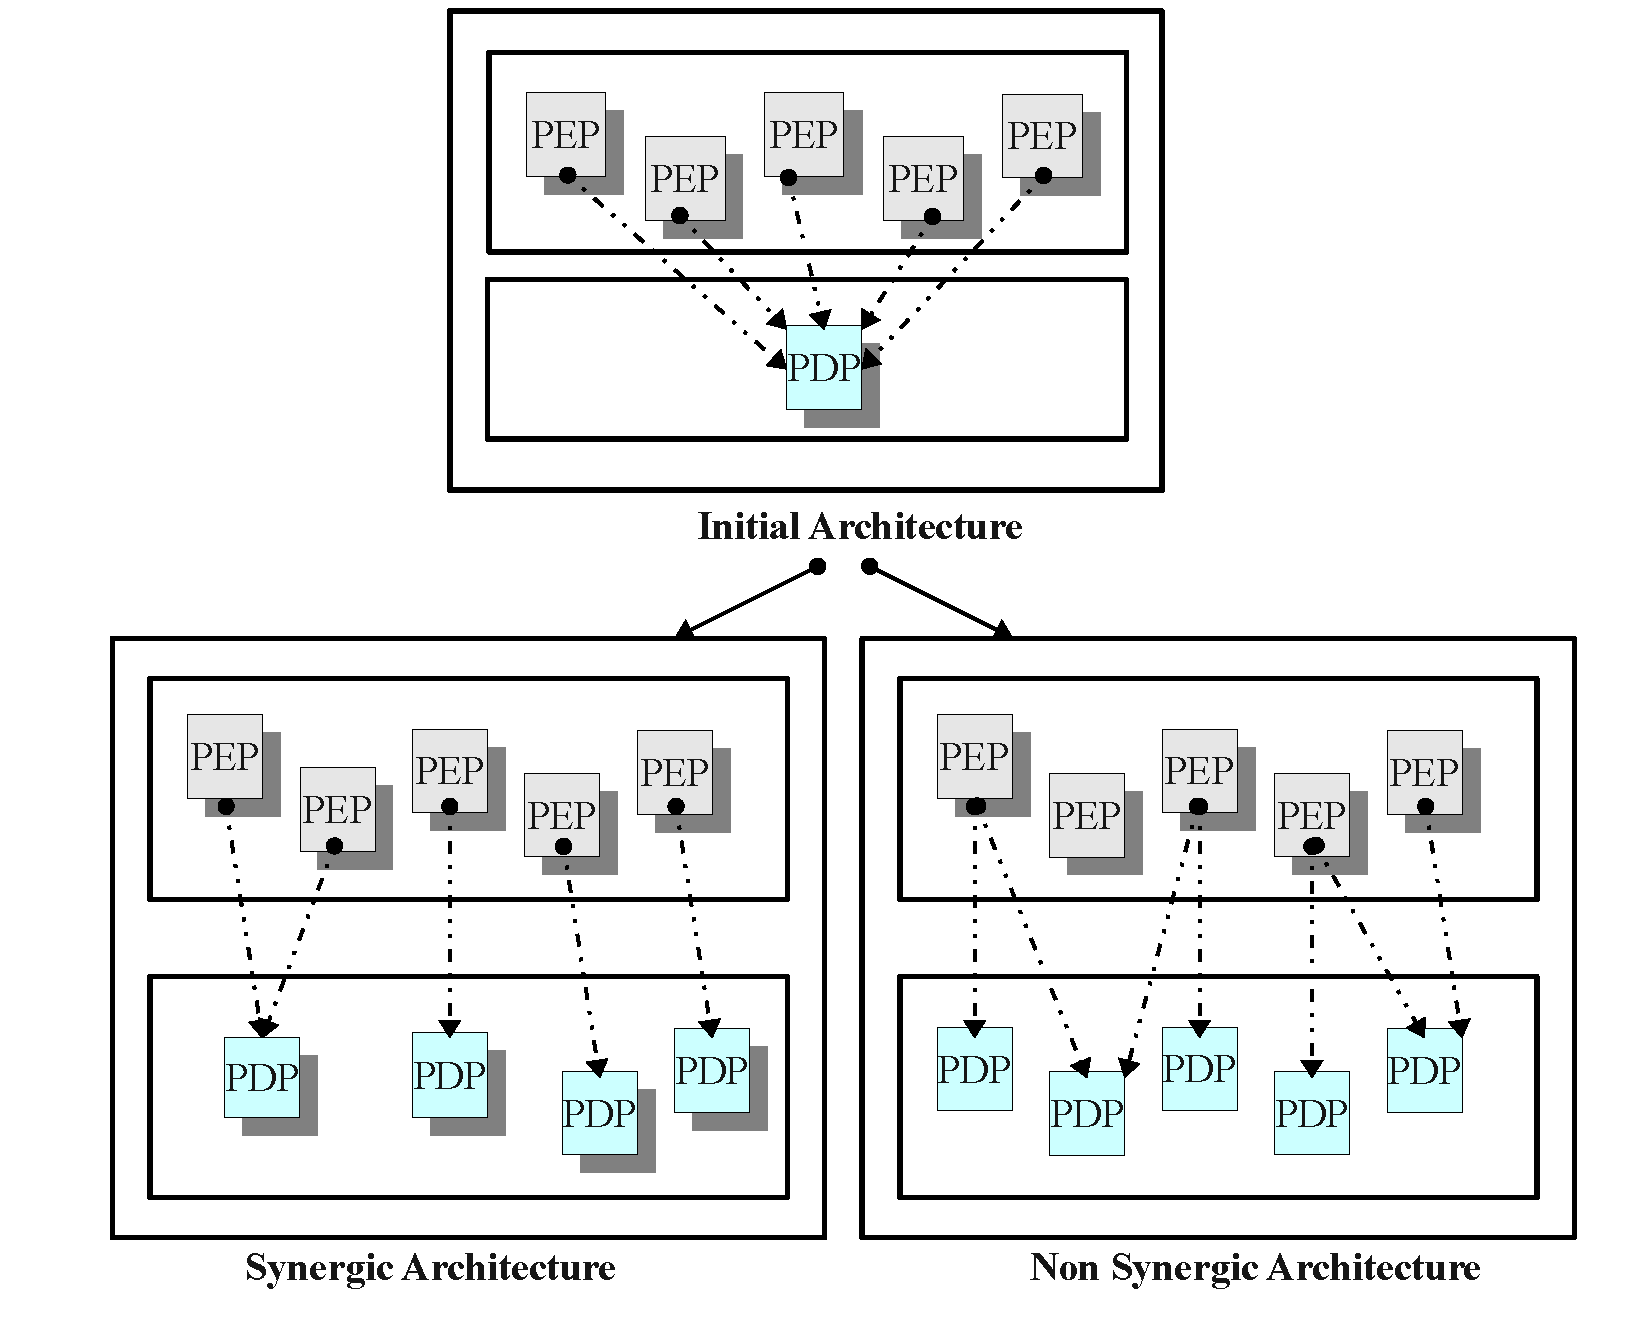
\includegraphics[width=8.5cm, height=6cm]{synergic-nonsynergic}
\caption{Synergic vs Non synergic System}
\label{Synergicvsnonsynergicarchitecture}
\end{center}
\end{figure}

At the application level, the PEP is represented by a method call that triggers a decision making process.
Figure \ref{PEPdeploymentexample} presents sample PEP code from our previous work in \cite{legacy}. This code snippet
 shows an example of a PEP 
represented by the method \CodeIn{checkSecurity}, which calls a method of the class \CodeIn{SecurityPolicyService}, which formulates a request to invoke the PDP component. 
The PEP represented by the method \CodeIn{ServiceUtils.checkSecurity} may issue requests that have subject ''user`` along fixed action 
and resource (``LibrarySecurityModel.BORROWBOOK\_METHOD''), (``LibrarySecurityModel.BOOK\_VIEW'').
Consider that we refactor a policy using $SC_{2}=\langle Resource,Action\rangle$, $SC_{1}=\langle Action\rangle$ or $SC_{1}=\langle Resource\rangle$.
Given a request issued from the PEP, our approach runs a PDP loaded with a policy containing rules sharing the same action and resource attribute values. 
Thus the splitting process that preserves the mapping between the PEPs and the PDP is the one that considers the following splitting criteria: 
$SC_{2}=\langle Resource,Action\rangle$, $SC_{1}=\langle Action\rangle$ and $SC_{1}=\langle Resource\rangle$ in this case.
In the evaluation section, we investigate the impact of the synergy property on performance.

\begin{figure}[!h]
\begin{center}
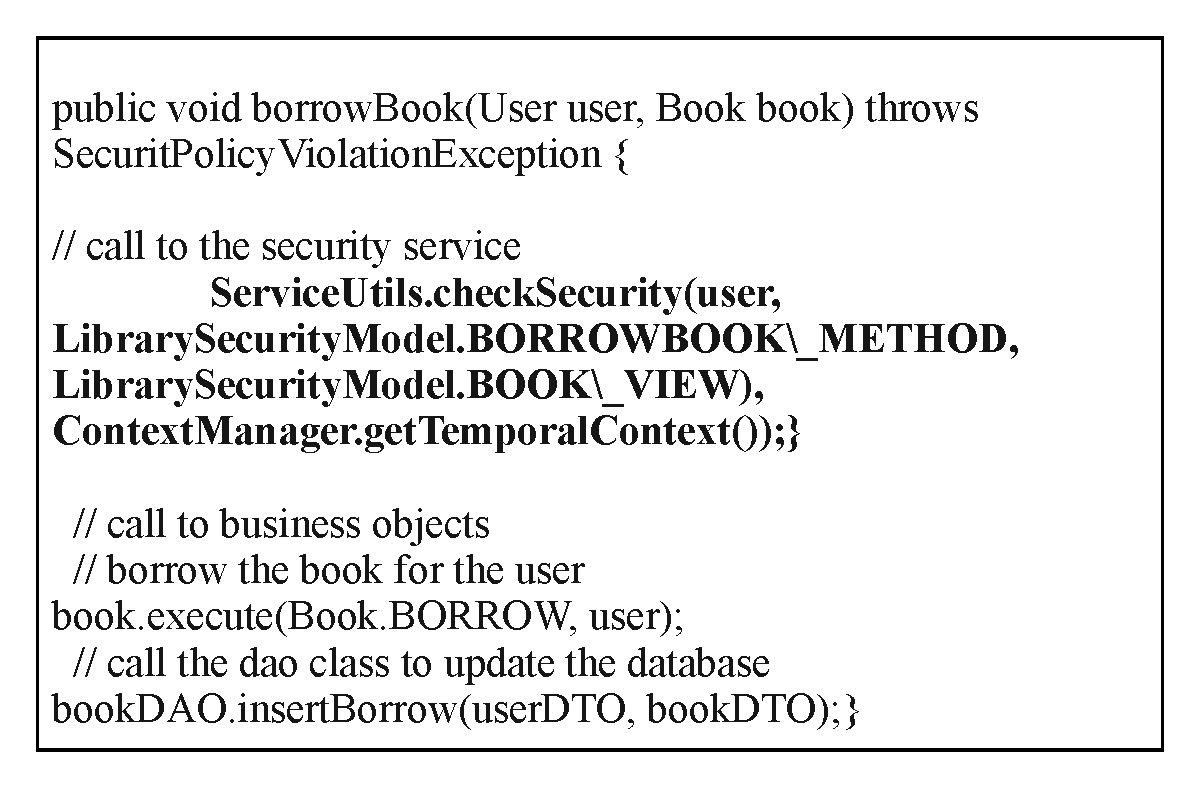
\includegraphics[width=7.5cm, height=4cm]{PEPExample}
\caption{PEP Deployment Example}
\label{PEPdeploymentexample}
\end{center}
\end{figure}